\documentclass[]{politex}

% ========== Packages ==========

\usepackage[utf8]{inputenc}
\usepackage{amsfonts}
\usepackage{amsmath}
\usepackage{amssymb}
\usepackage{amsthm}
\usepackage{amsthm}
\usepackage{booktabs}
\usepackage{float}
\usepackage{glossaries}
\usepackage{graphicx}
\usepackage{hyperref}
\usepackage{makecell}
\usepackage{subcaption}

% ========== Behavior Trees ==========

\usepackage[external]{forest}
\usepackage{xcolor}

\usetikzlibrary{arrows.meta}

\definecolor{GreenAction}{rgb}{0.702,0.941,0.702}
\definecolor{YellowCondition}{rgb}{0.98,0.941,0.431}
\definecolor{PurpleDecorator}{rgb}{0.8,0.8,1}

\forestset{
  controlflow/.style={draw, black, rectangle, minimum height=12mm, minimum width=12mm},
  decorator/.style={draw, fill=PurpleDecorator, diamond, minimum height=11mm, minimum width=11mm},
  action/.style={draw, fill=GreenAction, rectangle, minimum height=15mm, minimum width=25mm},
  condition/.style={draw, fill=YellowCondition, ellipse, minimum height=15mm, minimum width=19mm},
  subtree/.style={draw, fill=lightgray, rectangle, minimum height=15mm, minimum width=25mm},
  default preamble={
    for tree={
        semithick,
        font=\footnotesize,
        edge={semithick, -{Stealth}},
        l sep+=12pt,
        align=center,
        anchor=center,
        child anchor=north,
    },
  },
}

\def \root {\Large{$\mathbf{\varnothing}$}}
\def \fallback {\Large{$\mathbf{?^*}$}}
\def \reactivefallback {\Large{$\mathbf{?}$}}
\def \sequence {\Large{$\mathbf{\rightarrow^*}$}}
\def \reactivesequence {\Large{$\mathbf{\rightarrow}$}}
\def \parallel {\Large{$\mathbf{\rightrightarrows}$}}

\tikzexternalize[prefix=tikz/]

% ========== Language options ==========
% \usepackage[brazil]{babel}
\usepackage[english]{babel}

% ========== References ==========

\usepackage{csquotes}
\usepackage[style=abnt-numeric,sorting=none]{biblatex}
\addbibresource{references.bib}

% ========== Opções do documento ==========

\graphicspath{ {./images/} }
\makeglossaries
%\input{chapters/glossario.tex}

% Título
\titulo{A multi-agent strategy for coordinating a robot soccer team}

% Autor
\autor{Lucas Haug}

% Orientadora / Coorientador
\orientadora{Anarosa Alves Franco Brandão}
\coorientador{Arthur Henrique Casals do Nascimento}

% Tipo de documento
\tcc{Electrical}{with emphasis on Computing}

% Departamento e área de concentração
\departamento{Computer and Digital Systems Engineering}
\areaConcentracao{Computer Engineering}

% Local
\local{São Paulo}

% Ano
\data{2022}


\begin{document}
% ========== Capa e folhas de rosto ==========
\capa
\falsafolhaderosto
\folhaderosto

% ========== Folha de assinaturas (opcional) ==========
% \begin{folhadeaprovacao}
% 	\assinatura{Anarosa Alves Franco Brandão}
% \end{folhadeaprovacao}

% ========== Ficha catalográfica ==========
% Fazer solicitação no site:
%	http://www.poli.usp.br/en/bibliotecas/servicos/catalogacao-na-publicacao.html

% ========== Dedicatória (opcional) ==========
%\dedicatoria{Dedicatória}

% ========== Agradecimentos ==========
%\begin{agradecimentos}

%\end{agradecimentos}

% ========== Abstract ==========
\begin{abstract}
\def \MOISEp {$\mathcal{M}OISE^+$} 

In the academic world, university robotics competitions play a major role in developing the field of robotics both nationally and internationally, encouraging research and design of robotic systems. In the context of these competitions, one of the most challenging and stimulating robot categories is the \textit{IEEE Very Small Size Soccer (VSSS)}, which aims to develop a complete engineering solution for a team of robots that play soccer autonomously. The ThundeRatz Robotics Team at at the Polytechnic School of the University of São Paulo currently has a solution to the problem proposed by the category, which uses the \textit{Robotic Operating System (ROS)} to structure the system and behavior trees for modeling of intelligent agents who play soccer. This solution is known as the ThunderVolt team and will be the target of this work, which aims to improve the team by developing a specification of an organization of a multi-agent system based on the \MOISEp specification, using behavior trees. This organization will allow the elaboration of a team coordination strategy based on the technologies already used and validating these enhancements in an academic competition, the \textit{IRONCup 2023} \footnote{https://events.robocore.net/ironcup-2023/}.

%
\\[3\baselineskip]
%
\textbf{Keywords} IEEE Very Small Size Soccer, Robots Soccer, Multi-agent System, Behavior Tree, ROS.
\end{abstract}

% ========== Resumo ==========
\begin{resumo}
\def \MOISEp {$\mathcal{M}OISE^+$} 

No mundo acadêmico, as competições universitárias de robótica têm um grande papel no desenvolvimento do cenário da área tanto no quadro nacional quanto no internacional, incentivando a pesquisa e a concepção de sistemas robóticos. No contexto dessas competições, uma das categorias de robôs mais desafiadora e estimulante é a \textit{IEEE Very Small Size Soccer (VSSS)}, que visa desenvolver uma solução completa de engenharia para um time de robôs que jogam futebol autonomamente. A Equipe ThundeRatz de Robótica da Escola Politécnica da USP possui atualmente uma solução para o problema proposto pela categoria, a qual utiliza o \textit{Robotic Operating System (ROS)} para estruturação do sistema, árvores de comportamento para modelagem dos agentes inteligentes que jogam futebol e uma Máquina de Estados Finita para coordenar esses agentes. Essa solução é conhecida como o time ThunderVolt e é o alvo deste trabalho, o qual tem como objetivo aprimorar o time ao desenvolver uma uma nova estratégia de coordenação usando árvores de comportamento, tendo como base um modelo da organização do time feito usando \MOISEp. Além disso, o desempenho a melhoria foi comparado ao sistema anterior usando uma Máquina de Estados Finita e em uma competição acadêmica de robótica, os resultados de ambos os testes serão discutidos.
%
\\[3\baselineskip]
%
\textbf{Palavras-Chave} IEEE Very Small Size Soccer, Futebol de Robôs, Sistemas Multiagentes, Árvores de Comportamento, ROS.
\end{resumo}

% ========== Listas (opcional) ==========
\listadefiguras
\listadetabelas

% ========== Listas definidas pelo usuário (opcional) ==========
%\input{chapters/listaDeSimbolos.tex}

% ========== Sumário ==========
\sumario

% ========== Elementos textuais ==========

\chapter{Introduction}

\section{Motivation}

From robots used for the automation of industrial processes to personal assistants robots and exploring robots for areas of difficult access, in the robotics area, we observe several applications with approaches from the least to the most complex in order to solve the most varied problems. Therefore, in order to develop the most distinct solutions, robotics appears as a multidisciplinary field, covering different lines of research, such as artificial intelligence, electronics, control, embedded systems, among many others.

One of the most prominent areas today is mobile robots, which aim to solve more complex tasks, in which the robot needs to move to carry out its activities. The difficulty of this branch is in how to control and coordinate the actions of robots so that they can interact with the environment and achieve their goal. For the accomplishment of some tasks, only one robot is not enough, being necessary then to use multiple robots, which makes the system more complex. Such systems prove how it is indispensable to have a control architecture for the coordination of all robots and a model of the organization of the system, capable of managing all the tasks that robots must perform, in order to achieve the system's objective, as can be seen in \cite{ACMultiplosRobos} and \cite{Moise}.

At the same time, in the line of development of control architectures for modeling intelligent agents in robotics, one of the fronts is the use of behavior trees to build the behavior of intelligent agents. Behavior trees were already widely used in the game development scenario, for modeling the behavior of non-playable characters, and, thanks to their modularity and flexibility, they have been gaining more and more notoriety in robotics \cite{BTsInRobotics}.

In this way, it is possible to take advantage of the structure provided by the behavior trees to model systems in which it is necessary to control the actions of several robots, being able to model both the behavior of the robots with behavior trees, as well as the organization that will coordinate all robots.

\section{Project Context}

\subsection{The ThundeRatz Robotics Team}

In order to develop national robotics and participate in academic competitions, the robotics team at Polytechnic School of the University of São Paulo was founded in 2001. This team, initially called \textit{Los Cuervos}, was reformed in 2005, giving rise to ThundeRatz \cite{ThundeRatz}.

Currently supervised by Prof. Dr. Rafael Traldi Moura, the group aims to learn about several topics that touch the state of the art of robotic systems, having contact with the newest lines of research. All this technical knowledge is used to design projects that encompass several areas of engineering, so that the team can put these projects to the test in national and international robotics competitions, gaining prominence on the robotics world stage.

At the moment, the team has several projects, having combat robots, sumo, hockey robots and autonomous robots that perform the most varied tasks, such as playing soccer or following a line on the ground.

\begin{figure}[!h]
    \centering
    \includegraphics[width=.6\linewidth]{images/ThundeRatz Logo.png}
    \caption{ThundeRatz's logo. Taken from \cite{ThundeRatz}}
\end{figure}

\subsection{The IEEE Very Small Size Soccer (VSSS) category}

One of the most challenging and stimulating academic robotics competition categories is the \textit{IEEE Very Small Size Soccer (VSSS)} category. In it, competitors must develop an engineering solution for a team of robots that must play soccer autonomously, with each team composed of three players, each with maximum dimensions of 75 mm x 75 mm x 75 mm. The match is played on a 130mm x 150mm field and consists of two game periods, each lasting five minutes, with a half-time break of ten minutes.

Originally, the category had only its version with physical robots, in which matches are played on a black field with white markings and the robots have colored markings on their top, so they can be identified by means of a camera located above the field. However, due to the COVID-19 pandemic, the category adapted to the health context and also started to occur in a simulated environment, using the FIRASim \cite{FIRASim} simulator.

For the physical version, in addition to game strategies, the teams need to develop the mechanical and electronic system of the robots, as well as a computer vision system to identify the positions and speeds of the robots in the field and a communication system between the computer that runs game strategy and physical robots, for the transmission of movement commands.

As for the simulated version, there is no need to develop the systems relate to the physical world, only the system to determine the game strategy and a communication interface with the game simulator and with an automatic judge \cite{VSSReferee} developed for the category.

\begin{figure}[!h]
    \centering
    \includegraphics[width=.7\linewidth]{images/General System.png}
    \caption{Representative scheme of the system used in the category. Taken from \cite{FutRobosFerramentaDeEnsino}}
    \label{fig:general_system}
\end{figure}

\subsection{The ThunderVolt Team}

To participate in the \textit{VSSS} category, the ThundeRatz team developed a team of robots called ThunderVolt \cite{ThunderVolt} \cite{TDPThunderVolt}.

For its physical version, four robots were developed, called: Alan, Dorothy, Grace and Alex. Each inspired by a figure in science and engineering, with the honorees being, respectively, Alan Turing, Dorothy Vaughan, Grace Hopper and Alessandro Volta. In addition, a computer vision system was developed, using the library \textit{OpenCV} \cite{OpenCV}, and a communication system with physical robots, through the radio frequency modules nRF24L01 and an open source library developed by team \cite{STM3232RF24}. For its simulated version, a communication interface with the simulator and the automatic judge was developed using the UDP protocol.

\begin{figure}[!ht]
    \centering
    \includegraphics[width=.6\linewidth]{images/ThunderVolt Robots.jpeg}
    \caption{ThunderVolt team physical robots. Taken from \cite{ThunderVolt}}
    \label{fig:physical_robots}
\end{figure}

Regarding the central system that determines the strategy of the game and controls the behavior of the robots, it was implemented using the \textit{Robotic Operating System (ROS)} \cite{ROS}, a framework that provides several tools and libraries useful for developing robotics applications. Furthermore, to coordinate the team's actions, different technologies were used, such as methods of navigation through vector fields \cite{VectorFields} and behavior trees \cite{BTsInRobotics} to determine the behavior of each robot.

\section{Objectives}

This work aims to improve the architecture, maintainability and performance of the ThunderVolt team, in the competitions of the \textit{VSSS} category of autonomous robot soccer. Therefore, the intention is to introduce a new cooperation strategy based on an organizational model \cite{Moise} of agents, using behavior trees to model the structure of the organization and using the behavior of the existing agents. Thus, the objective of this work will involve the central system for determining the team's strategy, without impacting the other systems used in the project.

\section{Justification}

The use of the state of the art organizational model \cite{Moise} in combination with the use of behavior trees, which are a trend in the field of robotics \cite{BTsInRobotics}, guarantee a great opportunities for improvements in the ThunderVolt team, making the system more flexible, scalable and modular, thus enabling an improvement in its performance.

\section{Project Organization}

This work is currently divided into four chapters, with this introduction being the first.

In Chapter \ref{ch:methodology}, the project methodologies to be used in this work will be detailed, indicating the activities to be carried out and the goals.

In Chapter \ref{ch:target_system}, it will be described how the target system, the ThunderVolt team, works prior to the proposed changes, describing its current structure and the way it responds to external commands.

Finally, in Chapter \ref{ch:requirements}, the requirements of the team improvement proposal will be described.

\def \MOISEp {$\mathcal{M}OISE^+$} 
\def \MOISEpBf {$\mathbf{\mathcal{M}OISE^+}$} 

\chapter{Background}
\label{ch:background}

This chapter explains the theoretical foundation for understanding this work, from the basics of multi-agent systems and modeling these systems to different control architectures used in robotics.

\section{Multi-agents systems}

a

\section{\MOISEpBf}

% exemplos

\section{Control Architectures}

%  - AC multiplos robos, ambientes dniamicos

% https://arxiv.org/pdf/1709.00084.pdf
% comparacao entre arquiteturas

\section{Finite State Machines}

\section{Hierarchical State Machines}

\section{Behavior Trees}

% https://www.overleaf.com/learn/latex/Algorithms

% arrumar ref na implementacao sobre reactive

% \linkhttps{https://en.wikipedia.org/wiki/Behavior_tree_(artificial_intelligence,_robotics_and_control)}
% https://www.overleaf.com/learn/latex/TikZ_package
% https://forum.thunderatz.org/t/arquiteturas-de-controle/3640
% https://www.behaviortree.dev/docs/learn-the-basics/BT_basics

\subsection{Types of Nodes}

\subsubsection{Root Node} 

\subsubsection{Control Nodes} 
\label{subsubsec:control_nodes}

\subsubsection{Action Nodes}

\subsubsection{Condition Nodes}

\subsubsection{Decorator Nodes}

\subsubsection{Subtree Nodes}

\subsection{Reactivity}

\subsection{Blackboard}


\cite{BlackboardDesignPattern}


\section{BT vs other Control Architectures}


\def \MOISEp {$\mathcal{M}OISE^+$} 

\chapter{Methodology}
\label{ch:methodology}

In order to develop the new strategy for the team based on an organizational model, the entire workflow of the project was subdivided into several distinct phases. These phases include the initial phases of the project, one cycle of work related to the definition of the specification of the new strategy, another cycle related to the implementation of the strategy, and the final phases of the work, as depicted in Figure \ref{fig:methodology}.

The initial phases of the project consisted of two parts. The first phase of the work was to carry out an analysis of the feasibility of adopting the \MOISEp \cite{MOISEp} model to better understand the system and to observe how a new strategy could be implemented. This analysis will be presented in Chapter \ref{ch:target_system}. After that, before starting the development of the project, the requirements for its implementation were listed, as will be seen in Chapter \ref{ch:requirements}.

The project followed a development cycle consisting of two phases: specification and implementation. The development started with the specification cycle, in which several iterations of the specification were performed to refine the specifications until the first implementable version was achieved. Once the initial specification was finalized, the implementation cycle began, which started with the implementation of the tree nodes. Then, with all tree nodes implemented, the first implementation of the team's strategy BT was assembled. 

The implemented BT was then used to test the system against the FSM-based system to ensure that the new system performed at least as well and could cover the same use cases. Finally, the tested system was submitted for review by the ThunderVolt team; this review was then used to fix some problems with the specification of the tree, starting the specification cycle all over again, and in other cases to fix implementation errors, starting the implementation cycle all over again. After many tests and revisions, a final version of the implementation was obtained, which was then merged into the team's main code branch. 

The detailed specification and implementation of the tree structure will be presented in Chapter \ref{ch:development}, while the results of the performance tests comparing the BT-based system with the FSM-based system will be discussed in Chapter \ref{ch:results}.

After finishing the system improvements, all changes were validated in an academic competition, the \textit{IRONCup 2023} \cite{IRONCup2023}, and the results of the competition will also be shown in Chapter \ref{ch:results}.

\begin{figure}
    \centering
    \includegraphics[width=\linewidth]{images/Methodology.png}
    \caption{Work methodology and development cycle}
    \label{fig:methodology}
\end{figure}


\chapter{Target System}
\label{ch:target_system}

\def \MOISEp {$\mathcal{M}OISE^+$}

To enable a better understanding of the proposed improvements, it is necessary to comprehend the functioning of the system prior to the changes. For this, the rules to which the system must obey and the organizational model used before the changes, following the structure of the \MOISEp \cite{MOISEp} model, will be explained and, based on these two factors, the previous game strategy will be presented.

\section{Game Rules}
\label{sec:rules}

In this section, the relevant rules for understanding the game strategy will be presented, the complete rules of the category can be accessed at \cite{RulesVSSS}.

During a match, several events can happen that influence the game strategy used, so the most important cases of the rules for the game strategy will be explained below. These events are sent to the team through the referee system developed for the category \cite{VSSReferee}, which uses the UDP protocol to send messages.

The events received from the referee system can be divided into two types, the game events and the control events. The game events are used to signalize something that happened in the game, for example, a foul, while the control events are used to indicate the flow of the game, as if the game is running or not.

The game events described in the rules are:

\begin{itemize}
    \item Free Kick: Event that occurs for specific types of fouls during the game, such as blocking the opponent's goalkeeper in his area, and which leads to a kick by the injured team from a certain marking on the field.
    \item Penalty: Event that covers different cases of fouls that are considered more serious, such as two robots inside the area actively defending the goal, and leads to a kick by the injured team from the penalty spot, towards the opponent's goal. This event can also occur for game tiebreakers.
    \item Goal Kick: Event that occurs, in general, when there is a foul in the attack, such as if two attacking robots enter the opposing team's goal area, and which results in a kick by the injured team, which can position the ball in any position within your goal area.
    \item Free Ball: Event that occurs when there is a deadlock and the ball is stopped for more than 10s outside the goal areas, that leads to a ball dispute, where the ball is positioned in the free ball marking of the quadrant in which it occurred.
    \item Kick off: Event that occurs when the game is started or restarted due to the occurrence of a goal. When this event occur, the ball is placed in the center of the field to be played. Depending on what happened in the event, one team will have repositioning priority over the other.
 \end{itemize}

Meanwhile, the control events are specified as follows:

\begin{itemize}
     \item Game On: Event that indicates that the game is running.
     \item Stop: Event that indicates that the game is not running.
     \item Halt: Event that occurs when the game is halted so that a human judge can verify an occurrence in the game and take the necessary actions. Upon receiving this event, the team must be able to return to the exact state it was when it received the event flag.
  \end{itemize}

\section{Organization Model}
\label{sec:organization_model}

Using the \MOISEp \cite{MOISEp} model, a mapping of the current solution was made, in order to validate the use of the model, facilitate the understanding of the current system and observe gaps for improvements, this mapping can be seen in Figure \ref{fig:moise_mapping}.

\begin{figure}[!ht]
    \centering
    \includegraphics[width=\linewidth]{images/ThunderVolt Moise-Structural Specification.png}
    \caption{Mapping of the solution to the MOISE model made by the author}
    \label{fig:moise_mapping}
\end{figure}

From the diagram, it is possible to better understand the functioning of the system, which will be detailed below.

The ThunderVolt team is made up of three robots, however, to ensure greater versatility in what each robot can do, seven possible roles were defined that robots can play, the roles and their responsibilities are defined as follows:

\begin{itemize}
    \item Goalkeeper: Defends the goal.
    \item Striker: Carries out attacks against the opposing team.
    \item Assistant: Positions itself strategically to take advantage of rebounds in the attack.
    \item Penalty Kicker: Kicks penalties in the opposing team.
    \item Penalty Defender: Defends the opposing team's penalties.
    \item Fullback: Helps the goalkeeper to defend the goal
    \item Wingback: Helps the defense, while trying to make counterattacks.
\end{itemize}

It is important to note that the behavior of these roles, meaning the way they perform these functions, has already been implemented using behavior trees prior to this work. This experience of using behavior trees to define the roles to be performed proved to be quite advantageous, due to the ease of implementation, flexibility and modularity.

Regarding the roles listed, some of these are played while the team is attacking and others while the team is defending. As not all roles can be performed simultaneously, there is an entity in the organization, called Coach, which is responsible for assigning each of the three robots a certain role in the game. As a game is a dynamic scenario, as time goes by it is necessary to perform role swaps between the robots, these swaps are also coordinated by the Coach and depend on the role that each robot is playing at the moment.

Thus, for a robot that is playing a certain role to play another role, there must be a compatibility between the two roles, for example, the attacker role is not compatible with the goalkeeper role, due to different positioning and functionalities, meanwhile, the assistant and attacker roles are compatible with each other, thanks to the high synergy between the two roles in the attack state.

In general, the roles of penalty kicker and defender are used only when a penalty event occurs, with the penalty kicker being used in place of the attacker and the penalty defender in the place of the goalkeeper. However, the team supports many penalty modes, thus there is also the case where a penalty can be kicked by an attacker or defended by the goalkeeper. In other moments of the game, while the team is defending, the roles of goalkeeper, fullback and wingback are used and while the team is attacking, the roles of goalkeeper, assistant and striker are usually used. Besides that, in some special moments of the game, an extra striker can be used in place of the assistant to make the team more offensive.

To implement the Coach and all the swaps between the roles, the current structure uses a finite state machine, which will be described in the next section.

\section{Game Strategy}

Bearing in mind the roles used and the compatibilities between them, which allows the swap of roles between the robots, a finite state machine was developed to define the game strategy. With the increasing complexity of the strategy, this solution proved to be non-scalable and not sustainable for the project, which is a major gap for improvements in the current system. The size of the strategy code significantly expanded, making it difficult for the FSM to accommodate and scale with the increased complexity.

\begin{figure}[!h]
    \centering
    \includegraphics[width=\linewidth]{images/BehaviorsController FSM.png}
    \caption{Finite State Machine of game strategy diagram made by the author}
    \label{fig:behaviors_controller_fsm}
\end{figure}

The current solution can be seen in Figure \ref{fig:behaviors_controller_fsm}. In the finite state machine, it is possible to observe that there are eight possible states for the system, three of which are states in which role swaps occur and the other five are input and waiting states. The determination of which state the state machine will start in is done in advance, upon receiving one of the events described in Section \ref{sec:rules}, for example, upon receiving a penalty event for the opposing team, the entry state will be the penalty defense state. Each transition between states is controlled by a guard function and when the condition of this function is satisfied, a transition function is called, all these functions are listed in Figure \ref{fig:behaviors_controller_fsm}.

An important feature to note is that in all cases, to go to a swap state, a swap condition is analyzed, meanwhile, to exit these states and return to the attack or defense states, the negation of the swap condition is analyzed. This is necessary to ensure that the swap state will only be exited when the swap is complete and cannot happen immediately afterward, guaranteeing a hysteresis to the system and avoiding multiple subsequent swaps that would make the system unstable.


\chapter{Requirements}
\label{ch:requirements}

This chapter presents the technical requirements for improving the system discussed in Chapter \ref{ch:target_system}.

This improvement will be based on the refinement of the organization of the multi-agent system, using behavior trees to describe all the entities of the system.

\section{Functional requirements}

For the development of the new game strategy based on a behavior tree, the new model must be able to cover all the use cases of the model that uses a finite state machine, dealing with the various events stated in Section \ref{sec:rules}.

Therefore, the model must be able to receive events from the referee, handle those events, control whether the robots should play or not, and most importantly, switch robot roles based on the current state of the game.

\section{Non-functional requirements}

When it comes to non-functional requirements, it is vital to ensure that all proposed changes do not adversely affect the team's performance in a game. Consequently, the team must maintain a comparable or improved level of performance.

Furthermore, for the changes to qualify as system improvements, the new strategy must improve maintainability, enhance the flexibility for changes and be easier to understand. These objectives can be specified by means of the following qualifications:

\begin{itemize}
    \item \textbf{Qualitative scalability}. From page 85 of \cite{MASScalability}:

    \begin{citacaoLonga}
    This is about (i) actors or agents with a more complex and richer inner life, i.e. with manifold interests and motives, abilities and features and advanced possibilities to build relationships to other actors or agents, or (ii) institutionalised behaviour patterns and regularities on different levels of sociality independent from special persons and interactions (like in organizations).
\end{citacaoLonga}

    \item \textbf{Quantitative scalability}. From page 85 of \cite{MASScalability}:

    \begin{citacaoLonga}
    This form refers to the size of the constellation under research (whether it is composed of human actors in a social context or artificial agents in a multiagent system). Hence, the focus is on mechanisms that help increasing population sizes to reproduce sociality, and social order.
    \end{citacaoLonga}

    \item \textbf{Modularity}. From page 6 of \cite{BTsInRobotics}:

    \begin{citacaoLonga}
    Modular design is an approach that subdivides a system into smaller parts or modules, that can be independently created and then used in different systems. A modular system can be characterized by functional partitioning into discrete and scalable modules. A modular design is loosely connected with code reusability and it can allow an heterogeneity of code developers’ expertise.
    \end{citacaoLonga}

    \item \textbf{Human readability}. From page 6 of \cite{BTsInRobotics}:

    \begin{citacaoLonga}
    A readable structure is desirable for reducing the cost of developing and debugging, especially when the task is human designed. The structure should remain readable even for large systems. Human readability requires a coherent and compact structure.
    \end{citacaoLonga}
\end{itemize}


\chapter{Development}
\label{ch:development}

This chapter will outline the developmental stages of the newly devised strategy for the project, encompassing the technologies employed and culminating in the final solution achieved.

\section{Specification}
\label{sec:specification}

Given the requirements presented in Chapter \ref{ch:requirements}, a specification for the Coach behavior tree was developed, which was called \texttt{Behaviors Controller} tree. Due to the complexity of the tree, the main tree was divided into subtrees, taking advantage of the modularity of the BTs. The following subsections will individually elaborate on each of the subtrees within the system, providing a detailed explanation for each. 

Furthermore, to be able to develop the tree, custom nodes were created, some that are shared between the trees and others more specific to each of the subtrees. To better organize the explanation of those nodes, the common nodes will be explained in the next subsection, while the specific nodes will be elucidated alongside the explanation of the subtrees they are part of.

\subsection{Common Nodes}
\label{subsec:common_nodes_spec}

First, to understand the developed specification for the tree, it is necessary to understand the common nodes used to build it.

\subsubsection{Root Node}

In all the following trees, the root node is represented as depicted in Figure \ref{fig:root_node_spec}.

\begin{figure}[!h]
    \centering
    \begin{forest}
        [\root, controlflow]
    \end{forest}
    \caption{Root node representation}
    \label{fig:root_node_spec}
\end{figure}

\subsubsection{Control Flow Nodes}
\label{subsubsec:control_nodes_spec}

Three types of control nodes were used in the project, they are the non-reactive fallback and the non-reactive and reactive sequence nodes, as represented in Figure \ref{fig:control_nodes_spec}.

\begin{figure}[!h]
    \centering
    \begin{subfigure}[b]{.32\linewidth}
        \centering
        \scalebox{.8} {
            \begin{forest}
                [\fallback, controlflow]
            \end{forest}
        }
        \caption{Non-reactive fallback}
    \end{subfigure}
    \hfill
    \begin{subfigure}[b]{.32\linewidth}
        \centering
        \scalebox{.8} {
            \begin{forest}
                [\sequence, controlflow]
            \end{forest}
        }
        \caption{Non-reactive sequence}
    \end{subfigure}
    \hfill
    \begin{subfigure}[b]{.32\linewidth}
        \centering
        \scalebox{.8} {
            \begin{forest}
                [\reactivesequence, controlflow]
            \end{forest}
        }
        \caption{Reactive sequence}
    \end{subfigure}
    \caption{Used control nodes representation}
    \label{fig:control_nodes_spec}
\end{figure}

\subsubsection{Action Nodes}
\label{subsubsec:common_action_nodes_spec}

From all the action nodes used in the trees, there are two types of action nodes that are common to the trees.

The first commonly used action node, depicted in Figure \ref{fig:always_success_action_node_spec}, is a simple node that always returns success when ticked. 

On the other hand, the second commonly used action node, illustrated in Figure \ref{fig:set_blackboard_action_node_spec}, is more complex. It is configured to assign an input value to an environment variable. This node is referred to as the \texttt{Set Blackboard} node, as it employs the blackboard pattern to facilitate the sharing of environment variables among nodes.

\begin{figure}[!h]
    \centering
    \begin{subfigure}[b]{.49\linewidth}
        \centering
        \scalebox{1.} {
            \begin{forest}
                [{Always Success}, action]
            \end{forest}
        }
        \caption{Always success}
        \label{fig:always_success_action_node_spec}
    \end{subfigure}
    \hfill
    \begin{subfigure}[b]{.49\linewidth}
        \centering
        \scalebox{1.} {
            \begin{forest}
                [{Set Blackboard \\ variable = value}, action]
            \end{forest}
        }
        \caption{Set Blackboard}
        \label{fig:set_blackboard_action_node_spec}
    \end{subfigure}
    \caption{Common used action nodes representation}
    \label{fig:common_action_nodes_spec}
\end{figure}

\subsubsection{Condition Nodes}
\label{subsubsec:common_condition_nodes_spec}

In a similar way to the \texttt{Set Blackboard} node, a common condition node used in the trees is a node called \texttt{Blackboard Check}. This node compares the value of a variable stored in the blackboard with a specified value, if both values are equal the node returns success, otherwise, it returns failure. The structure of the node can be seen in Figure \ref{fig:common_condition_node_spec}.

\begin{figure}[!h]
    \centering
    \scalebox{1.} {
        \begin{forest}
            [{Blackboard Check \\ variable == value}, condition]
        \end{forest}
    }
    \caption{\texttt{Blackboard Check} condition node representation}
    \label{fig:common_condition_node_spec}
\end{figure}

\subsubsection{Subtrees}
\label{subsubsec:subtrees_spec}

During the tree development process, in order to enhance the tree's modularity and comprehensibility, many subtrees were used in the specification. All the subtrees utilized are different, however, they share the same representation. The representation, shown in Figure \ref{fig:subtrees_spec}, is done by means of a node that acts as a placeholder for the complete specification of the subtree.

\begin{figure}[!h]
    \centering
    \scalebox{1.} {
        \begin{forest}
            [{Subtree}, subtree]
        \end{forest}
    }
    \caption{Subtree node representation}
    \label{fig:subtrees_spec}
\end{figure}

\subsection{Behaviors Controller Tree}

With a grasp of the nodes that are shared among the subtrees within the system, it is possible now to delve into the explanation of the main tree that defines the new game strategy, the \texttt{Behaviors Controller} tree.

During a match there are two distinguishable moments, the first when the ball is stopped, e.g. when a foul happened or simply when the game is starting, and the second when the ball is in motion. To be able to fully control the behavior of the team during a match, we need a strategy that handles both of these game moments. For this reason, the basic structure of the main tree was modeled as a sequence of two subtrees, a structure illustrated in Figure \ref{fig:behaviors_controller_bt_spec}. The sequence, in this case, is a non-reactive sequence, as the moments when the ball is stopped are much less common, so there is no need to reactively check if the game is stopped.

The first subtree in the sequence is the \texttt{Roles Swapper Initializer} subtree, responsible for performing the swapper initialization process. This initialization takes place whenever the system receives any of the events described in Section \ref{sec:rules}. Therefore this part of the tree handles the moments when the ball is stopped, preparing the system to be able to dynamically swap the roles of the robots. Following the initialization phase, the subsequent subtree to be ticked is named as \texttt{Roles Swapper}. This subtree is responsible for checking if there are any necessary role swaps between the robots and executing the corresponding changes accordingly.

\begin{figure}[!h]
    \centering
    \begin{forest}
        [\root, controlflow
            [\reactivesequence, controlflow  
                [{Roles Swapper \\Initializer Subtree}, subtree]
                [{Roles Swapper \\Subtree}, subtree]
            ]
        ]
    \end{forest}
    \caption{Base structure specification of the Coach’s Behavior Tree}
    \label{fig:behaviors_controller_bt_spec}
\end{figure}

\subsection{Roles Swapper Initializer}
\label{subsec:roles_swapper_initializer_spec}

As mentioned previously, this subtree is specifically designed to handle situations in the game when the ball is not in motion. The purpose of this subtree is to incorporate the initialization part of the system directly into the tree structure. This modeling approach was selected to make the system more concise and organized. By integrating the initialization process within the tree, the behavior tree gains better control over its execution flow. The final initializer tree can be seen in Figure \ref{fig:roles_swapper_initializer_spec}.

\begin{figure}[!h]
    \centering
    \resizebox{\columnwidth}{!} {
        \begin{forest}
            [\root, controlflow
                [\sequence, controlflow
                    [\fallback, controlflow
                        [\fallback, controlflow
                            [{Blackboard Check \\ game\_state == running}, condition]
                            [\sequence, controlflow
                                [{Set Blackboard \\ use\_penalty\_mode = False}, action]
                                [{Set Blackboard \\ use\_two\_strikers\_mode = False}, action]
                                [{Always Failure}, action]
                            ]
                        ]
                        [{Events Handler Subtree}, subtree]
                        [\sequence, controlflow
                            [{Blackboard Check \\ game\_state == halt}, condition]
                            [{All Roles are Set}, condition]
                        ]
                        [\sequence, controlflow
                            [{Set Blackboard \\ team\_state = attacking}, action]
                            [{Initialize Roles \\ By Position}, action]
                        ]
                    ]
                    [{Set Blackboard \\ game\_state = running}, action]
                ]
            ]
        \end{forest}
    }
    \caption{Roles Swapper Initializer subtree specification}
    \label{fig:roles_swapper_initializer_spec}
\end{figure}

The initialization tree was modeled so that while the game is running, the tree will returns success and nothing of the initialization will be done, otherwise, the initialization will be done, depending on the event received from the referee (described in Section \ref{sec:rules}) and at the end, the tree will return success as well. 

In order to handle the event received from the system, the event value is saved in a blackboard variable with the name \texttt{game\_state} and it is by using this variable that all initialization is performed. The value of the variable is set on the blackboard by an agent external to the tree, which is the one responsible for communicating with the referee and is not included in the strategy part of the Coach.

The base of the tree is a sequence of a fallback, which will be referenced as the primary fallback of this tree, and a final action node to ensure that at the end of the initialization, the game state is set to be \texttt{running}. 

The first child of the primary fallback is another fallback, referred to as the second fallback, which is responsible for checking if the game is running and, if it is not, starting the initialization phase. The initialization process is initiated by a sequence, the one that is the second child of the second fallback. This sequence resets some configuration variables and concludes by returning a failure. This failure is crucial to allow the primary fallback to proceed with the remaining steps of the initialization.

The second child of the primary fallback is a subtree called \texttt{Events Handler}, which will be better explained in the Subsection \ref{subsec:events_handler_spec}. The objective of this subtree is to handle the different kinds of \textbf{game events}, as specified in Section \ref{sec:rules}, and set the team configuration accordingly. If the subtree is not able to handle the received event, it returns a failure.

The third child of the primary fallback is a sequence, which is important in case the received event is the control event \texttt{Halt}. When a \texttt{Halt} is received, ideally all the robots' roles should remain the same, however, if for some reason there are robots with no role set, then a default initialization should be used. Therefore, this sequence returns success if a \texttt{Halt} was received and all the robots' roles are set and failure otherwise.

The last child of the primary fallback is the one responsible for the default initialization of the roles. If the system received any other event that was not handled or, as explained, if it receives a \texttt{Halt} and there are roles that are not set, then the system uses the default initialization, which is to attack and use the current robots' positions to initialize the roles.

Finally, it is important to specify a detail about this tree and all of its subtrees, which is that reactive control nodes are not used in them, since once the initialization is started, there is no need to run the already executed nodes again.

\subsection{Events Handler and its subtrees}
\label{subsec:events_handler_spec}

As described previously, the \texttt{Events Handler} subtree is responsible for managing the game events received from the referee. Its structure, depicted in Figure \ref{fig:events_handler_spec}, consists of a fallback with four subtrees, each designed to handle a specific event. Each of these subtrees then first verifies if the received event matches the event it is meant to handle, if it does, the subtree proceeds with the corresponding event-specific initialization, otherwise, it simply returns a failure.

It is important to note that, in Section \ref{sec:rules}, five game events were defined, however, from those five events, the \texttt{Events Handler} subtree only handles four, it does not handle the \texttt{Free Kick} event. Despite that event being specified in the rules of the category, it is never sent by the referee due to its complexity, so it is not necessary to handle it in the tree.

Another relevant piece of information about this subtree is that it does not set the initial roles of the robots, it just initializes the configurations for the \texttt{Roles Swapper} subtree. The initial roles of the robots are predefined values that are obtained from a configuration file, which defines arbitrarily for each robot an initial robot role and an initial position for each of the four game events handled by the \texttt{Events Handler} subtree.

\begin{figure}[!h]
    \centering
    \resizebox{0.7\columnwidth}{!} {
        \begin{forest}
            [\root, controlflow
                [\fallback, controlflow
                    [{Penalty Kick Event \\ Handler Subtree}, subtree]
                    [{Goal Kick Event \\ Handler Subtree}, subtree]
                    [{Free Ball Event \\ Handler Subtree}, subtree]
                    [{Kickoff Event \\ Handler Subtree}, subtree]
                ]
            ]
        \end{forest}
    }
    \caption{Events Handler subtree specification}
    \label{fig:events_handler_spec}
\end{figure}

\subsubsection{Penalty Kick Event Handler}

The \texttt{Penalty Kick Event Handler}, presented in Figure \ref{fig:penalty_kick_event_handler_spec}, deals with the case when a \textit{Penalty Kick} event was received. The tree first checks whether the game state event received was a \textit{Penalty Kick}, if it was, then an initialization sequence for the \textit{Penalty Kick} event is executed. 

\begin{figure}[!h]
    \centering
    \resizebox{0.6\columnwidth}{!} {
        \begin{forest}
            [\root, controlflow
                [\sequence, controlflow      
                    [{Blackboard Check \\ game\_state == penalty\_kick}, condition]
                    [\sequence, controlflow
                        [{Set Penalty Mode}, action]
                        [\fallback, controlflow
                            [\sequence, controlflow      
                                [{Blackboard Check \\ game\_state\_team == friends}, condition]
                                [{Set Blackboard \\ team\_state = attacking}, action]
                            ]
                            [{Set Blackboard \\ team\_state = defending}, action]
                        ]
                    ]
                ]
            ]
        \end{forest}
    }
    \caption{Penalty Kick Event Handler subtree specification}
    \label{fig:penalty_kick_event_handler_spec}
\end{figure}

The first child of this sequence is a node called \texttt{Set Penalty Mode}, which sets a blackboard variable named \texttt{use\_penalty\_mode}. This variable controls whether the penalty kicker role will be used in place of the attacker and whether the penalty defender role will be used in place of the goalkeeper. The variable value is set in the blackboard and can be either \texttt{True} or \texttt{False}, its value is determined based on some user configurations for the match, depending on the opposing team.

The second child of the sequence is a fallback. The structure built by this fallback and its children is used to check whether the penalty event received was for the friends' team and, if it was, set the \texttt{team\_state} blackboard variable to be \texttt{attacking}, otherwise set it to be \texttt{defending}. To know for which team the penalty event was, the \texttt{game\_state\_team} blackboard variable is checked, which is a variables updated using the data from the \textit{VSSReferee}.

\subsubsection{Goal Kick Event Handler}

The \texttt{Goal Kick Event Handler}, shown in Figure \ref{fig:goal_kick_event_handler_spec}, is responsible for the \textit{Goal Kick} event, as its name implies. Similarly to the \texttt{Penalty Kick Event Handler} subtree, this tree first checks whether the game event received was a \textit{Goal Kick} and executes the rest of the subtree in case it was.

\begin{figure}[!h]
    \centering
    \resizebox{.9\columnwidth}{!} {
        \begin{forest}
            [\root, controlflow
                [\sequence, controlflow      
                    [{Blackboard Check \\ game\_state == goal\_kick}, condition]
                    [\fallback, controlflow
                        [\sequence, controlflow      
                            [{Blackboard Check \\ game\_state\_team == friends}, condition]
                            [{Set Blackboard \\ team\_state = defending}, action]
                        ]
                        [\sequence, controlflow      
                            [{Set Blackboard \\ team\_state = attacking}, action]
                            [{Set Blackboard \\ use\_two\_strikers\_mode = True}, action]
                        ]
                    ]
                ]
            ]
        \end{forest}
    }
    \caption{Goal Kick Event Handler subtree specification}
    \label{fig:goal_kick_event_handler_spec}
\end{figure}

In contrast to the configuration performed by the \texttt{Penalty Kick Event Handler} subtree, in case the received goal kick event was for the friends' team, this subtree sets the \texttt{team\_state} to be \texttt{defending}. Meanwhile, in case it was for the opposing team, then two configurations are set, the first one specifies that the team will attack and the other forces the team to use two strikers instead of just one when the game resumes, in order to make the team more offensive.

\subsubsection{Free Ball Event Handler}

The \texttt{Free Ball Event Handler}, as illustrated in Figure \ref{fig:free_ball_event_handler_spec}, is very similar in terms of structure to the \texttt{Goal Kick Event Handler} subtree. The difference between these two trees, other than the \texttt{Free Ball Event Handler} subtree deals with \textit{Free Ball} events, is that while the \texttt{team\_state} in the \texttt{Goal Kick Event Handler} is defined based on which team the event was directed to, in the \texttt{Free Ball Event Handler}, the \texttt{team\_state} is defined depending on which side of the field the free ball event occurred, information obtained from the \texttt{game\_state\_side} blackboard variable, updated using the data from the \textit{VSSReferee}. In case the free ball event took place on the friends' side of the field, the team will defend, otherwise the team will attack and will use two strikers instead of one.

\begin{figure}[!h]
    \centering
    \resizebox{.9\columnwidth}{!} {
        \begin{forest}
            [\root, controlflow
                [\sequence, controlflow      
                    [{Blackboard Check \\ game\_state == free\_ball}, condition]
                    [\fallback, controlflow
                        [\sequence, controlflow      
                            [{Blackboard Check \\ game\_state\_side == friends}, condition]
                            [{Set Blackboard \\ team\_state = defending}, action]
                        ]
                        [\sequence, controlflow      
                            [{Set Blackboard \\ team\_state = attacking}, action]
                            [{Set Blackboard \\ use\_two\_strikers\_mode = True}, action]
                        ]
                    ]
                ]
            ]
        \end{forest}
    }
    \caption{Free Ball Event Handler subtree specification}
    \label{fig:free_ball_event_handler_spec}
\end{figure}

\subsubsection{Kickoff Event Handler}

The final specific event handler subtree, the \texttt{Kickoff Event Handler}, depicted in Figure \ref{fig:kickoff_event_handler_spec}, is the one responsible for handling the \textit{Kickoff} events. It is simpler than the other specific event handler subtrees, as it just checks if the game event received was a \textit{Kickoff} event, in the positive case, it defines the \texttt{team\_state} to be \texttt{attacking} if the event was directed to the friends' team and to be \texttt{defending} if it was directed to the opposing team.

\begin{figure}[!h]
    \centering
    \resizebox{0.6\columnwidth}{!} {
        \begin{forest}
            [\root, controlflow
                [\sequence, controlflow      
                    [{Blackboard Check \\ game\_state == kickoff}, condition]
                    [\fallback, controlflow
                        [\sequence, controlflow      
                            [{Blackboard Check \\ game\_state\_team == friends}, condition]
                            [{Set Blackboard \\ team\_state = attacking}, action]
                        ]
                        [{Set Blackboard \\ team\_state = defending}, action]
                    ]
                ]
            ]
        \end{forest}
    }
    \caption{Kickoff Event Handler subtree specification}
    \label{fig:kickoff_event_handler_spec}
\end{figure}

\subsection{Roles Swapper}
 
The tree that is, in fact, responsible for swapping the roles basically has two sub-branches, as can be seen in Figure \ref{fig:roles_swapper_spec}, the one on the left for the attack state and the other on the right for the defense state, which are the two children branches of the fallback in the root of the tree. 

In the attack sub-branch, the first node that is ticked is the node that checks whether the team is attacking or not, by verifying the value of the \texttt{team\_state} variable in the blackboard. If the team is attacking, then the rest of the attacking branch is executed, otherwise, the tree ticks the defense sub-branch.

Disregarding the part of the attacking sub-branch that checks whether the team is attacking or not, the two sub-branches have a very similar structure. These branches essentially verify whether the team should continue attacking/defending (using condition nodes), if so, the attack/defense internal swap subtrees are executed. In case the team should not continue to attack/defend, then the roles of the robots need to be changed from the attack roles to the defense roles, or from the defense roles to the attack roles. In addition, right after changing the roles, so the tree can check the current state of the team, the new state of the team must be set in the blackboard, by changing the value of the \texttt{team\_state} variable.

To swap the roles from one team state to another, the current role of each robot is analyzed and, based on the intra-group compatibility links between the roles (see Figure \ref{fig:moise_mapping}), a new role from the other state is assigned to the robot. For example, when switching from the defense state to the attack state, a robot playing the wingback role, will be assigned to play the striker role.

Lastly,  regarding the reactivity of this tree, most of the control nodes in this tree are non-reactive, while a few are reactive. The fallback node at the root, for instance, is non-reactive, as the attack sub-branch will only be executed again if the last node of the defense sub-branch is executed. The other non-reactive nodes in the tree were selected based on criteria such as their children not requiring re-ticking or their results remaining unchanged if ticked again. On the other hand, the two reactive nodes used were chosen to be reactive because the team needs to be responsive when transitioning from the attack state to the defense state and vice-versa.

\begin{figure}[!h]
    \centering
    \resizebox{\textwidth}{!} {
        \begin{forest}
            [\root, controlflow
                [\fallback, controlflow    
                    [\sequence, controlflow      
                        [{Blackboard Check \\ team\_state == attacking}, condition]
                        [\fallback, controlflow        
                            [\reactivesequence, controlflow          
                                [{Should Continue \\Attacking}, condition]
                                [{Attack Swapper \\Subtree}, subtree]
                            ]
                            [\sequence, controlflow 
                                [{Swap To \\Defense Roles}, action]
                                [{Set Blackboard \\ team\_state = defending}, action]
                            ]
                        ]
                    ]
                    [\fallback, controlflow        
                        [\reactivesequence, controlflow          
                            [{Should Continue \\Defending}, condition]
                            [{Defense Swapper \\Subtree}, subtree]
                        ]
                        [\sequence, controlflow 
                            [{Swap To \\Attack Roles}, action]
                            [{Set Blackboard \\ team\_state = attacking}, action]
                        ]
                    ]
                ]
            ]
        \end{forest}
    }
    \caption{Roles Swapper subtree specification}
    \label{fig:roles_swapper_spec}
\end{figure}
 
\subsection{Attack Swapper and Defense Swapper}

Finally, to carry out the role swaps between the attack roles when in the attack state or between the defense roles when in the defense state, two trees were developed, the \texttt{Attack Swapper} (Figure \ref{fig:attack_swapper_spec}) and the \texttt{Defense Swapper} (Figure \ref{fig:defense_swapper_spec}). 

\begin{figure}[!h]
    \centering
    \resizebox{\textwidth}{!} {
        \begin{forest}
            [\root, controlflow
                [\fallback, controlflow    
                    [\sequence, controlflow      
                        [{Blackboard Check \\use\_two\_strikers\_mode == True}, condition]
                        [\sequence, controlflow        
                            [{Change from Two Strikers \\to One Striker mode}, action]
                            [{Set Blackboard \\use\_two\_strikers\_mode = False}, action]
                        ]
                    ]
                    [\sequence, controlflow      
                        [{Blackboard Check \\use\_penalty\_mode == True}, condition]
                        [\sequence, controlflow        
                            [{Change Penalty \\Kicker to Striker}, action]
                            [{Set Blackboard \\use\_penalty\_mode = False}, action]
                        ]
                    ]
                    [{Swap Striker \\and Assistant}, action]
                    [{Always Success}, action]
                ]
            ]
        \end{forest}
    }
    \caption{Attack state internal swap subtree specification}
    \label{fig:attack_swapper_spec}
\end{figure}

\begin{figure}[!h]
    \centering
    \resizebox{0.8\textwidth}{!} {
        \begin{forest}
            [\root, controlflow
                [\fallback, controlflow    
                    [\sequence, controlflow      
                        [{Blackboard Check \\use\_penalty\_mode == True}, condition]
                        [\sequence, controlflow        
                            [{Change Penalty Defender \\to Goalkeeper}, action]
                            [{Set Blackboard \\use\_penalty\_mode = False}, action]
                        ]
                    ]
                    [{Swap Fullback \\and Wingback}, action]
                    [{Swap Goalkeeper \\and Wingback}, action]
                    [{Always Success}, action]
                ]
            ]
        \end{forest}
    }
    \caption{Defense state internal swap subtree specification}
    \label{fig:defense_swapper_spec}
\end{figure}

Both trees have similar working logic, only changing the types of role changes they perform. The purpose of these trees is to make the internal role changes of the attack and defense states, thus having several nodes that implement different changes. In the root of the two trees, non-reactive nodes wore used in order to improve the distribution of priorities between different role changes.

There are two types of nodes that can change the roles of the robots, the \textit{swap nodes} and the \textit{change nodes}. The difference between them is that the swap nodes perform changes between two robots, while the change nodes just change the role of one robot to another role. In both cases, the nodes internally analyze a condition to see if the role changes should be done and then return \texttt{failure} if the change was not performed, \texttt{running} if it is still being carried out and \texttt{success} if the change has been fully completed. Besides that, at the end of each tree, there is a node \texttt{Always Success}, so that, if no changes have taken place, these trees return \texttt{success} to indicate that all robots have the ideal role for the moment.

Furthermore, there are some branches of these trees, which include some specific role changes, which will only be executed when a certain configuration has been activated during initialization, that is, when the \texttt{Roles Swapper Initializer} tree has activated some configuration flag. Whenever the swaps related to these branches are completed, the flag is deactivated, preventing re-entry to these branches. The use cases covered by these configurations are the use of the penalty kicker and penalty defender roles, enabled by the use of the \texttt{use\_penalty\_mode} flag, and the use of two strikers in certain game moments, enabled by the use of the \texttt{use\_two\_strikers\_mode} flag.

It is important to note that all role changes presented in the trees are represented by the inter-groups compatibility links in Figure \ref{fig:moise_mapping}. For example, when the team is in the defense state, there may be a swap of roles between the robots playing the wingback and the fullback roles.


\section{Technologies Used}
\label{sec:technologies_used}

This Section will outline the technologies used to implement the BT specification detailed in Section \ref{sec:specification}.

\subsection{Behavior Trees Technologies}

\subsubsection{BehaviorTree.CPP}

Implementing a BT engine can be a complex task, when developing new BTs, the use of existing libraries is highly recommended. The use of libraries ensures greater ease in the development and debugging process, better quality of the developed code and greater support for features, in addition to having a community of developers who can help with software problems.

Regarding the use of libraries for developing BTs in robotics applications, there are two libraries that stand out \cite{BTsAndFSMApplications}, which are the \textit{BehaviorTree.CPP} \cite{BehaviorTree.CPP} and the \textit{PyTrees} \cite{PyTrees}. Both of these libraries have a huge community, many features and great documentation pages. 

As mentioned in Section \ref{sec:organization_model}, the ThunderVolt project already employed BTs, but for the implementation of the behaviors of the individual roles that the robots can play. In an older version of the project \cite{fira_thundervolt}, the team used the \textit{PyTrees} library to define the behavior of the roles, however, due to the computational intensity required by the project, the team had performance problems when using this library, which impaired its real-time reactivity. Therefore, as suggested by the \textit{PyTrees} documentation itself \cite{PyTreesDesign}, instead of using Python to model the trees, the team chose to migrate to the C++ language, in order to increase the system performance, hence the \textit{BehaviorTree.CPP} was used in that context.

The \textit{BehaviorTree.CPP} library presents a C++ framework to create BTs, providing tools that help develop many different and complex trees, extending the basic functionalities that BTs support. The library is an open-source project, which was initially maintained by the author of \cite{BTsInRobotics} and now is mainly maintained by Davide Faconti\footnote{https://github.com/facontidavide}.

The \textit{BehaviorTree.CPP} offers many features such as built-in nodes that simplify the process of implementing BTs, easy access to a well structured blackboard, asynchronous nodes, and many others. In addition, to enhance the development and debugging process of implementing BTs, the library provides a logging and profiling infrastructure to, for example, visualize and record the state transitions of the tree. Furthermore, one of its main advantages is the ability to describe trees using an interpreted language based on XML and create the trees dynamically during run-time, making the development process of the tree much faster, as changes in the tree can be easily implemented and tested.

Thus, this library presented itself as a great candidate to be used in the development of the new strategy for many reasons. One of the first reasons is the prior experience with the library, which significantly facilitated its usage for implementing the new strategy and provided an opportunity to evaluate the library's compatibility with the project's requirements. Besides that, the library presents many functionalities that are useful for the specified tree, in addition to being an open-source project, having a large community of developers using and supporting it and being extensively used in very diverse and important robotics applications, such as the Navigation 2 \cite{nav2}. 

Finally, it is important to mention that the tree was implemented with version 3.8 of the library, which was the latest version at the time of its development. There are already newer versions of the library, but changing to these newer versions would not impact the structure of the presented tree.

\subsubsection{Groot}
\label{subsubsec:groot}

When it comes to building and debugging BTs, having a visual tool that allows visualizing the tree structure and facilitates tracking the execution flow of the tree proves to be immensely beneficial. Hence, another tool compliant with the \textit{BehaviorTree.CPP} library was developed by Davide Faconti, called \textit{Groot} \cite{Groot}.

\textit{Groot} is an integrated development environment for BTs that were developed with \textit{BehaviorTree.CPP}, which offers the possibility to visually edit and export trees, record the execution flow of a tree in a log file and replay it afterward, and monitor each tick of the tree in real-time.

This tool is one of the other advantages of using the \textit{BehaviorTree.CPP} library and was used during the whole process of development and debugging of the new strategy.

It is important to note that there are two versions of \textit{Groot} currently available. The first version is an open-source project, compatible with version 3.8 of the \textit{BehaviorTree.CPP} library and unfortunately it is being deprecated at the moment. The second version of \textit{Groot} has more advanced functionalities and it supports version 3.8 and versions equal to or higher than 4.2 of the library, however, it is no longer an open-source project and most of its features require a paid license.

\begin{figure}[h]
    \centering
    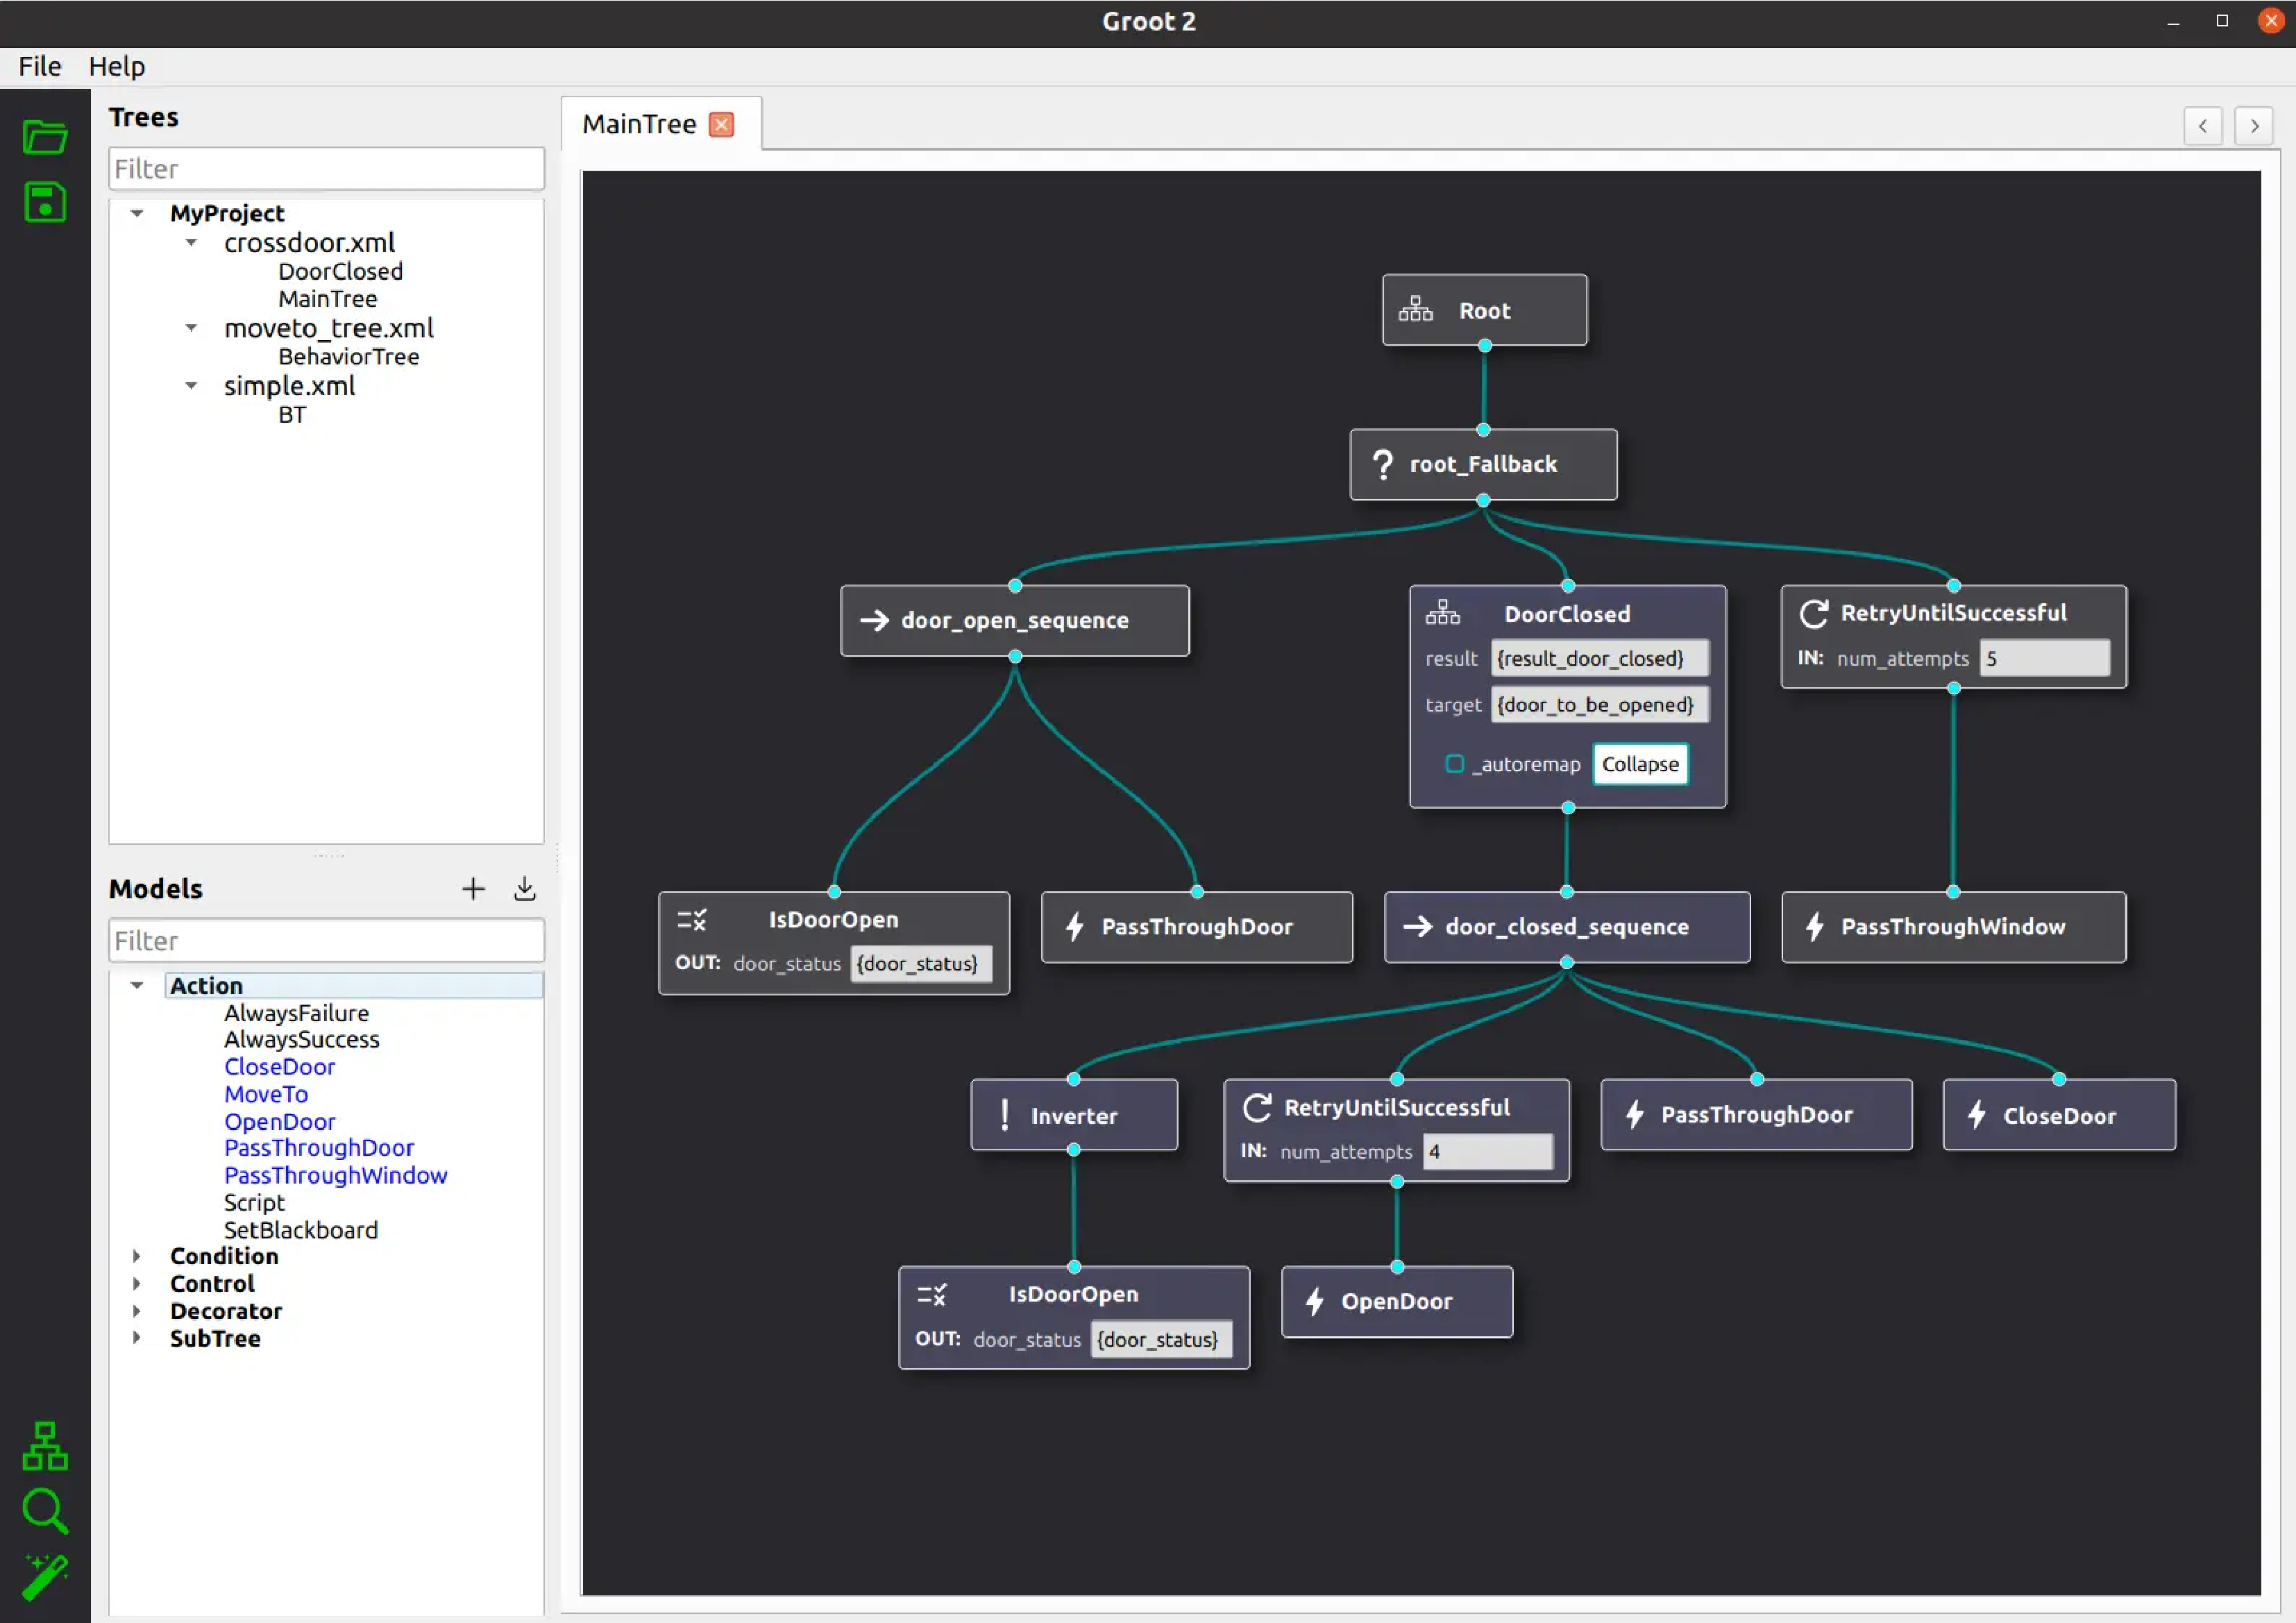
\includegraphics[width=0.75\linewidth]{images/Groot.pdf}
    \caption{Groot 2 interface. Taken from \cite{Groot}}
    \label{fig:groot}
\end{figure}

\subsection{Auxiliary Technologies}

In addition to the technologies used to build and debug the trees, other technologies are utilized in the context of the tree's operation, which will be elucidated as follows. These technologies were not chosen during the development of the new strategy, they were already employed by the ThunderVolt project and are part of its architecture as a whole.

Within this Subsection, these other technologies will be presented and their integration within the tree will be elucidated. This detailed explanation aims to facilitate a comprehensive understanding of how the tree is integrated with the rest of the system.

\subsubsection{Protobuf and UDP}

In the VSSS category, there are two tools that are important when testing and playing games, which are the FIRASim \cite{FIRASim}, a simulator used in the category, and the VSSReferee \cite{VSSReferee}, an automatic referee system which sends the game state and game control events to the teams playing a match. Both of these systems are crucial for the operation of the tree, as the simulator sends the states of the robots, which are used to decide when the roles of the robots should change, and the referee sends the events that define when the \texttt{Roles Swapper Initializer} tree (defined in Subsection \ref{subsec:roles_swapper_initializer_spec}) should be executed and how the initialization should be performed. 

In order to be able to communicate with those two systems, a protocol was defined by the category \cite{VSSProto} using Google's Protocol Buffers (\textit{Protobuf}) \cite{Protobuf}. The \textit{Protobuf} is a language-neutral and cross-platform framework to serialize data, so it can be stored or sent over a network. In the use case of the category, the serialized data is exchanged between the simulator, the referee and the teams playing the game using the User Datagram Protocol (UDP) \cite{rfc768}. The UDP is one of the core communication protocols of the internet, being a transaction oriented protocol, meaning that it does not require the network nodes to establish a connection to be able to communicate with each other. For the UDP-based communication, the team leveraged the capabilities of the \textit{Boost.Asio} library \cite{BoostAsio}, which is a cross-platform C++ library for network communication.

\subsubsection{ROS}

The Robot Operating System (\textit{ROS}) \cite{ROS} is a framework for developing robotics applications, it offers a diverse set of libraries and tools that help to build robotics projects. \textit{ROS} has a very large and global community, which helps to maintain all the libraries and to develop new algorithms, drivers and tools for the framework.

In the ThunderVolt project, \textit{ROS} is used to compose the structure of the whole software application, defining how the project will be executed, specifying the communication interface between all the different parts of the project that are performed in parallel, in addition to helping the system to be easily configurable and calibrated. In a less abstract way, for example, it is through ROS that the tree that is running in a separate process publishes the roles of the robots to the other processes that represent the robots, so they can execute the correct behavior.


\section{Implementation}
\label{sec:implementation}

This section will detail the implementation of the specification described in Section \ref{sec:specification}, highlighting the differences between what was previously specified and the final implementation.

Similar to Section \ref{sec:specification}, this section will first present the nodes that are common to some trees, then each subtree of the strategy tree will be briefly introduced and any implementation details will be elucidated. All images of nodes and trees shown in this section were created using the \textit{Groot 2} interface (see Subsubsection \ref{subsubsec:groot}).

\subsection{Common Nodes}
\label{subsec:common_nodes_impl}

The common nodes presented in this section are mostly very similar to the nodes presented in the Subsection \ref{subsec:common_nodes_spec}, changing just their representation. However, due to implementation details of the \textit{BehaviorTree.CPP} library, some of the nodes changed drastically and these changes will be clarified.

\subsubsection{Root Node}

The root node is represented as shown in Figure \ref{fig:root_node_impl}.

\begin{figure}[!h]
    \centering
    \includegraphics[width=0.15\linewidth]{chapters/development/images/RootNode.png}
    \caption{Root node in \textit{Groot}}
    \label{fig:root_node_impl}
\end{figure}

\subsubsection{Control Flow Nodes}

In contrast to the representation of control flow nodes discussed in Subsubsection \ref{subsubsec:control_nodes_spec}, the default behavior of a control flow node in the \textit{BehaviorTree.CPP} library is to be non-reactive. Therefore, as can be seen in Figure \ref{fig:control_nodes_impl}, nodes that deviate from this default behavior are specified as reactive nodes, rather than marking the non-reactive nodes differently. 

However, it is important to note that the \texttt{Sequence} node in this implementation differs slightly from the non-reactive sequence presented in Chapter \ref{ch:background}. When one of its children returns a failure, instead of ticking it again the next time the sequence is ticked, the whole sequence is restarted. The library also provides a sequence node with the same behavior of the sequence with memory as presented in Chapter \ref{ch:background}, but it was not used in the implementation of the tree. 

Additionally, another type of control flow node was used in the tree implementation, which is the decorator node, however, the reason why this node was used in the tree implementation will not be explained in this subsubsection, but in Subsubsection \ref{subsubsec:decator_nodes_impl}.

\begin{figure}[!h]
    \centering
    \begin{subfigure}[b]{.32\linewidth}
        \centering
        \includegraphics[width=0.52\linewidth]{chapters/development/images/FallbackNode.png}
        \caption{Non-reactive fallback}
    \end{subfigure}
    \hfill
    \begin{subfigure}[b]{.32\linewidth}
        \centering
        \includegraphics[width=0.57\linewidth]{chapters/development/images/SequenceNode.png}
        \caption{Non-reactive sequence}
    \end{subfigure}
    \hfill
    \begin{subfigure}[b]{.32\linewidth}
        \centering
        \includegraphics[width=0.8\linewidth]{chapters/development/images/ReactiveSequenceNode.png}
        \caption{Reactive sequence}
    \end{subfigure}
    \caption{Used control nodes representations in \textit{Groot}}
    \label{fig:control_nodes_impl}
\end{figure}

\subsubsection{Action Nodes}

The implementation of the common action nodes, in Figure \ref{fig:common_action_node_impl}, is very similar to the specification presented in Subsubsection \ref{subsubsec:common_action_nodes_spec}, the \texttt{Always Success} node is precisely the same and the node that sets a variable in the blackboard is a little bit different. 

In the tree specification, all blackboard variables were represented as strings or booleans, however, in the implementation, some of those variables were created as integer variables instead, therefore, two nodes that store variables in the blackboard were used, one that stores strings and another that stores integers. These two nodes have the same syntax, in the node, the \texttt{value} field receives the value to be stored in the blackboard and the \texttt{output\_key} receives the name of the variable in which the value will be stored. One thing important to note is that the node in Figure \ref{fig:set_blackboard_string_impl} is a built-in node of the library, while the node in Figure \ref{fig:set_blackboard_int_impl} is a custom node inspired by the node from the library.

\begin{figure}[!h]
    \centering
    \begin{subfigure}[b]{.32\linewidth}
        \centering
        \includegraphics[width=0.7\linewidth]{chapters/development/images/AlwaysSuccessNode.png}
        \caption{Always success}
    \end{subfigure}
    \hfill
    \begin{subfigure}[b]{.32\linewidth}
        \centering
        \includegraphics[width=0.85\linewidth]{chapters/development/images/SetBlackboardIntNode.png}
        \caption{Set Blackboard Int}
        \label{fig:set_blackboard_int_impl}
    \end{subfigure}
    \hfill
    \begin{subfigure}[b]{.32\linewidth}
        \centering
        \includegraphics[width=0.85\linewidth]{chapters/development/images/SetBlackboardStringNode.png}
        \caption{Set Blackboard String}
        \label{fig:set_blackboard_string_impl}
    \end{subfigure}
    \caption{Common used action nodes representation in \textit{Groot}}
    \label{fig:common_action_node_impl}
\end{figure}

\subsubsection{Condition Nodes}

In contrast to the tree specification, the common condition node specified in Subsubsection \ref{subsubsec:common_condition_nodes_spec} was not used in the tree implementation, decorator nodes were used instead, as it will be explained in the next subsubsection.

\subsubsection{Decorator Nodes}
\label{subsubsec:decator_nodes_impl}

The tree specification was created using condition nodes that verify whether the content of a variable in the blackboard is equal to a specified value, returning success or failure depending on the result of the assessment. However, the \textit{BehaviorTree.CPP} library does not provide a built-in condition node with the described behavior, instead, the library offers decorators that can be used for the same purpose.

Two decorators from the library were used to substitute the condition nodes, the \texttt{Blackboard Check Int}, in Figure \ref{fig:blackboard_check_int_impl}, and the \texttt{Blackboard Check String}, in Figure \ref{fig:blackboard_check_string_impl}. Both these nodes are very similar, they compare a value A with a value B, if both values are equal, this node will return the same status of its child otherwise it will return the value specified in the "return\_on\_mismatch" field. The difference between these two decorators is just the variable type that they handle, as the first handles integers and the second strings. One important thing to note is how these nodes actually access variables' values in the blackboard. This is accomplished by specifying the variable's name using the syntax \texttt{\{variable\_name\}}. By employing this syntax, the variable's value will be substituted during the comparison process, so it can be compared to the value in the other field.

\begin{figure}[!h]
    \centering
    \begin{subfigure}[b]{.49\linewidth}
        \centering
        \includegraphics[width=0.65\linewidth]{chapters/development/images/BlackboardCheckIntNode.png}
        \caption{Blackboard Check Int}
        \label{fig:blackboard_check_int_impl}
    \end{subfigure}
    \hfill
    \begin{subfigure}[b]{.49\linewidth}
        \centering
        \includegraphics[width=0.65\linewidth]{chapters/development/images/BlackboardCheckStringNode.png}
        \caption{Blackboard Check String}
        \label{fig:blackboard_check_string_impl}
    \end{subfigure}
    \caption{Blackboard Check decorator nodes representation in \textit{Groot}}
    \label{fig:common_decorator_nodes_impl}
\end{figure}

Regarding the use of these decorators, as it is not possible to simply replace a condition node with a decorator, it was necessary to make changes to the structure of the tree specification where the condition nodes which check the blackboard were used. To implement these modifications, an analysis of the structure which utilizes the \texttt{Blackboard Check} as a condition node was conducted, leading to the development of two alternative approaches using the \texttt{Blackboard Check} decorator implementation of the library.

Considering the tree specification, all the use cases of the \texttt{Blackboard Check} as a condition node can be abstracted as the two structures in Figure \ref{fig:blackboard_check_eq_condition_node}. The first structure, Figure \ref{fig:blackboard_check_eq_condition_node_fall}, represents the cases where the condition node is used as the first child of a non-reactive fallback, whereas the second structure, Figure \ref{fig:blackboard_check_eq_condition_node_seq}, represents the cases where the parent node of the condition node is a non-reactive sequence instead.

\begin{figure}[!h]
    \centering
    \begin{subfigure}[b]{.49\linewidth}
        \centering
        \scalebox{0.74} {
            \begin{forest}
                [\root, controlflow
                    [\fallback, controlflow
                        [{Blackboard Check \\ variable == value}, condition]
                        [{Conditional Action}, action]
                    ]
                ]
            \end{forest}
        }
        \caption{\texttt{Blackboard Check} as a condition node in a fallback}
        \label{fig:blackboard_check_eq_condition_node_fall}
    \end{subfigure}
    \hfill
    \begin{subfigure}[b]{.49\linewidth}
        \centering
        \scalebox{0.74} {
            \begin{forest}
                [\root, controlflow
                    [\sequence, controlflow
                        [{Blackboard Check \\ variable == value}, condition]
                        [{Conditional Action}, action]
                    ]
                ]
            \end{forest}
        }
        \caption{\texttt{Blackboard Check} as a condition node in a sequence}
        \label{fig:blackboard_check_eq_condition_node_seq}
    \end{subfigure}
    \caption{Tree structures abstraction when using the \texttt{Blackboard Check} as a condition node}
    \label{fig:blackboard_check_eq_condition_node}
\end{figure}

The first alternative to use the described decorator instead of the condition node can be seen in Figure \ref{fig:blackboard_check_eq_action_in_sequence}, in which the condition node is replaced by a decorator configured to return failure when there is a mismatch in the comparison and to return its child status, which will always be a success, when there is a match, mimicking the behavior of the condition node. This approach can be used as an alternative to both cases presented in Figure \ref{fig:blackboard_check_eq_condition_node}.

The second alternative, illustrated in Figure \ref{fig:blackboard_check_eq_action_as_child}, is a less verbose approach, using the decorator in a more standard manner, instead of using it to mimic the behavior of a condition node. As this solution requires fewer nodes than the first alternative, it presents itself as a better option. However, this approach cannot be used for both cases depicted in Figure \ref{fig:blackboard_check_eq_condition_node}, as its behavior only corresponds to the behavior of the structure in Figure \ref{fig:blackboard_check_eq_condition_node_seq}.

Therefore, the tree implementation, which will be presented in the next subsections, was structured in a way to adapt the tree specification using these alternatives. In the tree specification parts where the structure depicted in Figure \ref{fig:blackboard_check_eq_condition_node_fall} was utilized, the alternative approach illustrated in Figure \ref{fig:blackboard_check_eq_action_in_sequence} was employed to simulate a condition node. Conversely, in the parts where the structure depicted in Figure \ref{fig:blackboard_check_eq_condition_node_seq} is present, the alternative approach from Figure \ref{fig:blackboard_check_eq_action_as_child} was utilized.

\begin{figure}[!h]
    \centering
    \begin{subfigure}[b]{.49\linewidth}
        \centering
        \includegraphics[width=0.85\linewidth]{chapters/development/images/BlackboardCheck - Equivalence 1.png}
        \caption{\texttt{Blackboard Check} as a decorator with conditional action in sequence}
        \label{fig:blackboard_check_eq_action_in_sequence}
    \end{subfigure}
    \hfill
    \begin{subfigure}[b]{.49\linewidth}
        \centering
        \includegraphics[width=0.85\linewidth]{chapters/development/images/BlackboardCheck - Equivalence 2.png}
        \caption{\texttt{Blackboard Check} as a decorator with conditional action as child}
        \label{fig:blackboard_check_eq_action_as_child}
    \end{subfigure}
    \caption{Equivalent tree structures when using the \texttt{Blackboard Check} node}
    \label{fig:blackboard_check_equivalences}
\end{figure}

\subsubsection{Subtrees}

The representation of a subtree in the \textit{BehaviorTree.CPP} library, shown in Figure \ref{fig:subtrees_impl}, is very similar to the subtree specification described in the Subsubsection \ref{subsubsec:subtrees_spec}. The only notable difference between the two is that the library's implementation has an attribute called \texttt{\_\_shared\_blackboard}, which is used to specify whether the subtree will have its own blackboard or whether the tree which includes this subtree will share its blackboard with the subtree. In addition, the representation of a subtree node in \textit{Groot} also has a button that can be used to expand the subtree node and view the entire subtree.

\begin{figure}[!h]
    \centering
    \begin{subfigure}[b]{.49\linewidth}
        \centering
        \includegraphics[width=0.6\linewidth]{chapters/development/images/SubtreeNode - Not Shared BB.png}
        \caption{Subtree without shared blackboard}
    \end{subfigure}
    \hfill
    \begin{subfigure}[b]{.49\linewidth}
        \centering
        \includegraphics[width=0.6\linewidth]{chapters/development/images/SubtreeNode - Shared BB.png}
        \caption{Subtree with shared blackboard}
    \end{subfigure}
    \caption{Subtree node representation in \textit{Groot}}
    \label{fig:subtrees_impl}
\end{figure}

\subsection{Behaviors Controller Tree}

The \textit{Behaviors Controller} tree implementation, disregarding its subtrees, is basically the same as its specification, as it is possible to observe in Figure \ref{fig:behaviors_controller_bt_impl}, being the only notable difference the fact that it is now made explicit in the trees that they have a shared blackboard, by setting the \texttt{\_\_shared\_blackboard} attribute to true.

\begin{figure}[!h]
    \centering
    \includegraphics[width=0.7\linewidth]{chapters/development/images/BehaviorsController.png}
    \caption{Base structure implementation of the Coach’s Behavior Tree}
    \label{fig:behaviors_controller_bt_impl}
\end{figure}

\subsection{Roles Swapper Initializer}

In the implementation of the \texttt{Roles Swapper Initializer} tree, modifications were made to the tree specification, taking into account the information provided about the common nodes in Subsection \ref{subsubsec:common_action_nodes_spec}. The resulting implementation is depicted in Figure \ref{fig:roles_swapper_initializer_impl}. It is important to note that there is one implementation detail in this tree that deviates from its original specification, which is the data types of the variables stored in the blackboard.

\begin{figure}[!h]
    \centering
    \includegraphics[width=1.0\linewidth]{chapters/development/images/RolesSwapperInitializer.png}
    \caption{Roles Swapper Initializer subtree specification}
    \label{fig:roles_swapper_initializer_impl}
\end{figure}

In this tree and its subtrees, six blackboard variables are manipulated, which are the \texttt{game\_state}, the \texttt{game\_state\_team}, the \texttt{game\_state\_side}, the \texttt{use\_penalty\_mode}, the \texttt{use\_two\_strikers\_mode} and the \texttt{team\_state}.

In the tree specification, the \texttt{game\_state}, the \texttt{game\_state\_team}, and the \texttt{game\_state\_side} variables were all presented as strings for simplifications reasons, however, none of the real messages received from the \textit{VSSReferee} use strings to represent these data, just integers (see Tables \ref{tab:referee_events_ids}, \ref{tab:target_team_event_codification} and \ref{tab:field_side_event_codification}), therefore, the type of these variables in the blackboard was changed to integer.

The \texttt{use\_penalty\_mode} and the \texttt{use\_two\_strikers\_mode} variables were previously declared as booleans, nevertheless, to take advantage of the formerly developed \texttt{Set Blackboard Int} node, their data types were changed to integers as well, being \texttt{0} equivalent to \texttt{False} and \texttt{1} to \texttt{True}.

The last variable, the \texttt{team\_state}, did not have its data type changed, it remained a string as it is an internal variable of the tree, and keeping it as a string simplifies the tree and makes it more understandable.

\begin{table}[!htbp]
    \centering
    \begin{tabular}{c c}
        \toprule
        Event Name   & Value \\
        \midrule
        Free Kick    & 0     \\
        Penalty Kick & 1     \\
        Goal Kick    & 2     \\
        Free Ball    & 3     \\
        Kickoff      & 4     \\
        Stop         & 5     \\
        Game On      & 6     \\
        Halt         & 7     \\
        \bottomrule
    \end{tabular}
    \caption{Integer identifications of the events sent by the \textit{VSSReferee}, see \cite{VSSProto}}
    \label{tab:referee_events_ids}
\end{table}

\begin{table}[!htbp]
    \centering
    \begin{tabular}{c c}
        \toprule
        Target Team & Value \\
        \midrule
        Friends     & 0     \\
        Foes        & 1     \\
        \bottomrule
    \end{tabular}
    \caption{Codification, using the event and the team color, of the target team of the event received from the \textit{VSSReferee}}
    \label{tab:target_team_event_codification}
\end{table}

\begin{table}[!htbp]
    \centering
    \begin{tabular}{c c}
        \toprule
        Side of field & Value \\
        \midrule
        Friends' side & 0     \\
        Foes' side    & 1     \\
        \bottomrule
    \end{tabular}
    \caption{Codification, using the event and the team color, of the side of the field in which the event received from the \textit{VSSReferee} occurred}
    \label{tab:field_side_event_codification}
\end{table}

\subsection{Events Handler and its subtrees}

The \texttt{Events Handler} subtree has the same structure as its specification, being the only difference that it specifies the \texttt{\_\_shared\_blackboard} attributes of its subtrees. The implementation can be seen in Figure \ref{fig:events_handler_impl}.

\begin{figure}[!h]
    \centering
    \includegraphics[width=1.0\linewidth]{chapters/development/images/EventsHandler.png}
    \caption{Events Handler subtree implementation}
    \label{fig:events_handler_impl}
\end{figure}

Considering the changes presented in Subsection \ref{subsec:common_nodes_impl} and the changes to the data types of the variables on the blackboard, the implementations of all subtrees of the \texttt{Events Handler} subtree are analogous to their specifications. The implementations of the four subtrees are represented in Figures \ref{fig:penalty_kick_event_handler_impl}, \ref{fig:goal_kick_event_handler_impl}, \ref{fig:free_ball_event_handler_impl} and \ref{fig:kickoff_event_handler_impl}.

One simple implementation detail that deserves attention is the presence of parameters in the \texttt{Set Penalty Mode} node in the \texttt{Penalty Kick Event Handler}. These parameters were added to the node so it could be more generic, instead of having those values hardcoded into the node's code.

\begin{figure}[!h]
    \centering
    \includegraphics[width=0.7\linewidth]{chapters/development/images/PenaltyKickEventHandler.png}
    \caption{Penalty Kick Event Handler subtree implementation}
    \label{fig:penalty_kick_event_handler_impl}
\end{figure}

\begin{figure}[!h]
    \centering
    \includegraphics[width=0.9\linewidth]{chapters/development/images/GoalKickEventHandler.png}
    \caption{Goal Kick Event Handler subtree implementation}
    \label{fig:goal_kick_event_handler_impl}
\end{figure}

\begin{figure}[!h]
    \centering
    \includegraphics[width=0.9\linewidth]{chapters/development/images/FreeBallEventHandler.png}
    \caption{Free Ball Event Handler subtree implementation}
    \label{fig:free_ball_event_handler_impl}
\end{figure}

\begin{figure}[!h]
    \centering
    \includegraphics[width=0.65\linewidth]{chapters/development/images/KickoffEventHandler.png}
    \caption{Kickoff Event Handler subtree implementation}
    \label{fig:kickoff_event_handler_impl}
\end{figure}

\subsection{Roles Swapper}

Taking into account the insights discussed in Subsection \ref{subsec:common_nodes_impl}, the implementation of the \texttt{Roles Swapper} tree adheres closely to its specification, as depicted in Figure \ref{fig:roles_swapper_impl}.

\begin{figure}[!h]
    \centering
    \includegraphics[width=1.0\linewidth]{chapters/development/images/RolesSwapper.png}
    \caption{Roles Swapper subtree implementation}
    \label{fig:roles_swapper_impl}
\end{figure}

\subsection{Attack Swapper and Defense Swapper}

Finally, the \texttt{Attack Swapper} and \texttt{Defense Swapper} subtrees were also implemented taking into account the modifications discussed in Subsection \ref{subsec:common_nodes_impl}, the results are illustrated in Figures \ref{fig:attack_swapper_impl} and \ref{fig:defense_swapper_impl}, respectively.

Regarding the implementation of the nodes in both of these trees, it is noteworthy how the nodes that perform the roles changes and swaps were developed. To enhance the performance of the trees, these nodes were developed as asynchronous nodes, specifically using coroutines as their foundation. This design choice allows the role changes to be executed in parallel with the rest of the tree, without blocking its execution. The use of coroutines to develop the nodes was possible thanks to the \textit{BehaviorTree.CPP} library, which provides many ways of creating asynchronous nodes.

\begin{figure}[!h]
    \centering
    \includegraphics[width=1.0\linewidth]{chapters/development/images/AttackSwapper.png}
    \caption{Attack state internal swap subtree implementation}
    \label{fig:attack_swapper_impl}
\end{figure}

\begin{figure}[!h]
    \centering
    \includegraphics[width=1.0\linewidth]{chapters/development/images/DefenseSwapper.png}
    \caption{Defense state internal swap subtree implementation}
    \label{fig:defense_swapper_impl}
\end{figure}



\chapter{Results}

\section{Comparison between models}

This differs from the previous system with the FSM, where the initialization process occurred outside the FSM during the definition of the FSM's entry state.

flags use penalty mode, use two strikers

These configurations were modeled in the FSM as entry states, however, in the behavior tree they were adapted as flags, being able to be activated and deactivated.

\section{Tests and Evaluation}

% numero de testes
% setup de testes
% statisticas
% jogos

\section{Discussion}

% ṕerformance pelo menos igual

In order to compare the performance of the system that uses a finite state machine with the system that uses a behavior tree to model the organization, all other parts of the system must be kept unchanged. This is necessary so that test games can be made, where the two systems with different strategies would face each other, so that some game metrics can be collected for statistical comparison of the solutions, comparing metrics such as ball possession, number of goals, time in each quadrant of the field, among others.

falar sobre os requisitos


\chapter{Final Considerations}
\label{ch:final_considerations}

\section{Conclusions}
% Apresentar o balanço do trabalho: resultados atingidos e não atingidos, com justificativas.

\section{Contributions}
% Apresentar as contribuições do trabalho, ressaltando o que foi efetivamente da autoria da equipe

\section{Continuity Prospects}
% Descrever os trabalhos que podem ser realizados como continuação do projeto de formatura. 

% ========== Glossário & Referências ==========

% \nocite{*}

\printbibliography
\printglossaries

% ========== Apêndices (opcional) ==========
%\input{chapters/apendice.tex}

\end{document}
